\chapter{Conception}
\label{ch:conception}

\section{La base de donnée}
\label{sec:database}
Comme des probes requests, des images, et des données personnelles vont être enregistrées et que du traitement
logique leur sera associé, il est important de concevoir une base de donnée claire et bien structurée.

\subsection{Modèle entité-association}
Plusieurs versions du modèle EA ont été imaginée avant d’arriver à la version finale. Afin de mieux cerner les enjeux
de la structure de la base de donnée, ces dernières vont être commentées. Mais d’abord, listons les différentes
entités

Vendor : Il s’agit du fabricant qui possède un OUI. Étant unique, cet identifiant servira comme clé de la table.

MACAddress : Représente une adresse MAC. Un booléean lui est associé pour savoir si elle semble aléatoire. Une
adresse MAC étant unique (ou presque) elle est utilisée comme clé de la table

Probe : Représente une probe request. L’heure à laquelle elle a été capturée ainsi que le SSID visé font partis de
l’entité.

Place : Représente l’endroit où la capture a eu lieu.

Picture : Représente une photo prise par le module caméra

Identity : Représente l’identité d’une personne. On y trouvera les données personnelle récupérée via différents
vecteurs.

\subsubsection{Première version}
Dans cette première ébauche, toutes les entités sont reliées de manière plutôt simpliste. Regardons toutefois
quelques-unes de ces relations.
Une entité « vendor » peut n’avoir délivré aucune adresse MAC puisqu’ils seront tous inséré dans la base de donnée
à sa création.

Dans ce modèle, une « Identity » est reliée à aucune ou plusieurs MACAddress et photo. (L’individu peut posséder
plusieurs appareils et plusieurs photo ont pu être prise)

\begin{figure}[H]
	\centering
	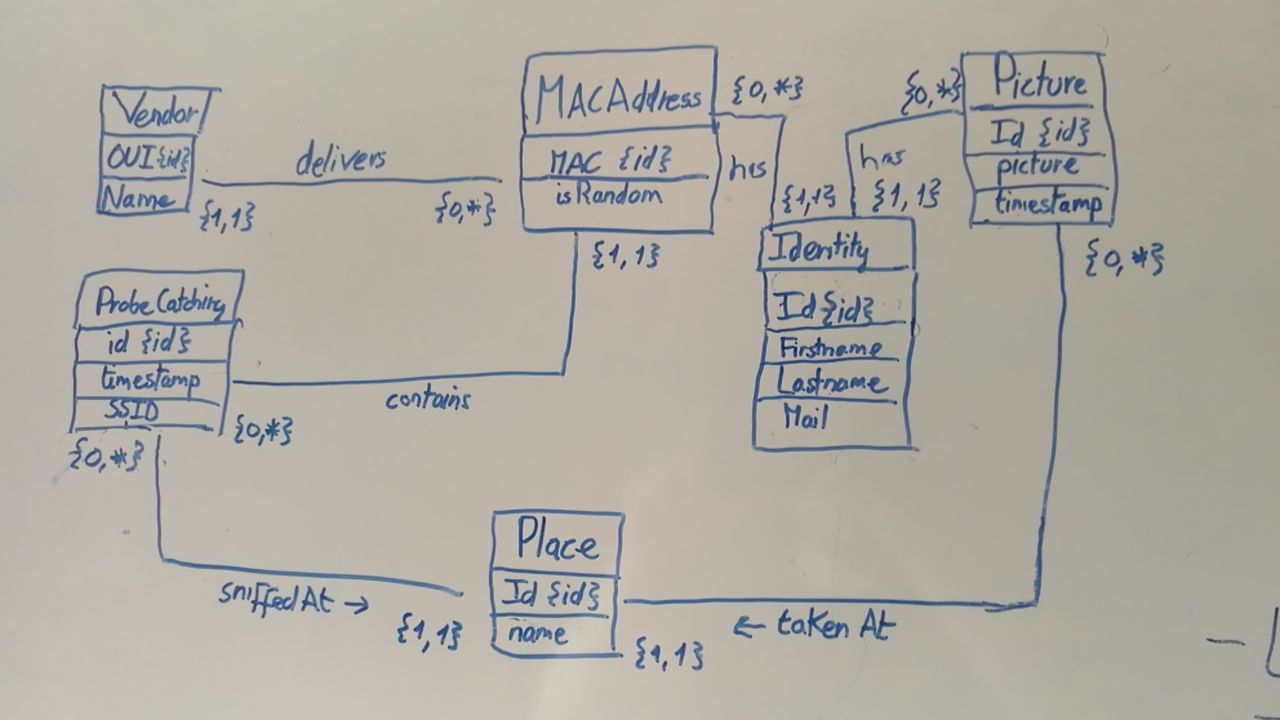
\includegraphics[width=12cm]{images/proto-1.png}
	\caption{Première version entité-association}
	\label{fig:arealytics}
\end{figure}

Problème : Dans cette conception, il n y a aucune notion de probabilité. Quand une identité a été reliée à une
adresse MAC par exemple, il n’est pas possible de modéliser le doute. Or, dans notre projet, il n y aura que très
peu d’occurence où la certitude est présente. Il faut donc modéliser cette propriété de probabilité.

\subsubsection{Deuxième version – Modélisation des probabilités}
Des relations intermédiaires ont été ajoutées. L’association entre une adresse MAC ou une photo avec une
identité est maintenant « pondérée » par une probabilité.

\begin{figure}[H]
	\centering
	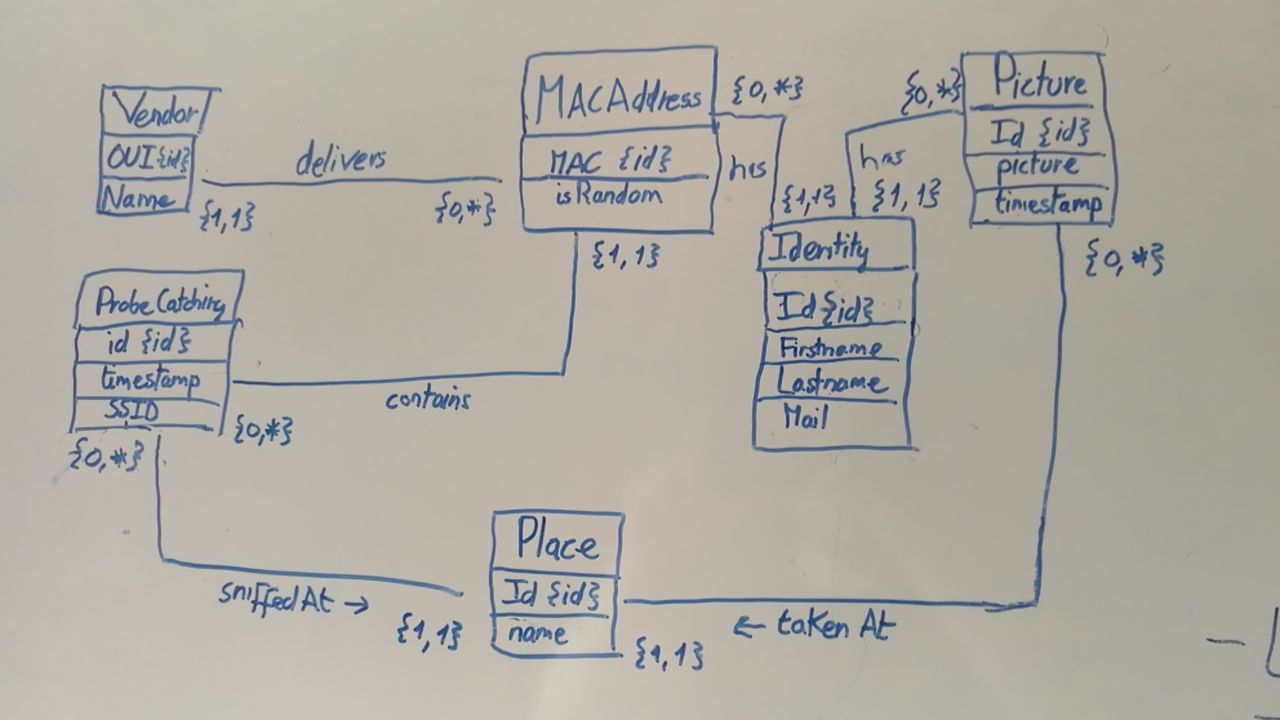
\includegraphics[width=12cm]{images/proto-1.png}
	\caption{Deuxième version entité-association}
	\label{fig:arealytics}
\end{figure}

Nouveau problème : Dans ce schéma, il est possible d’obtenir une identité sans image. Or, d’après les
spécifications, ce n’est pas possible puisque c’est grâce à la recherche inversée qu’une identité est établie.

\subsubsection{Troisième version – Identité à partir d’une photographie}

\begin{figure}[H]
	\centering
	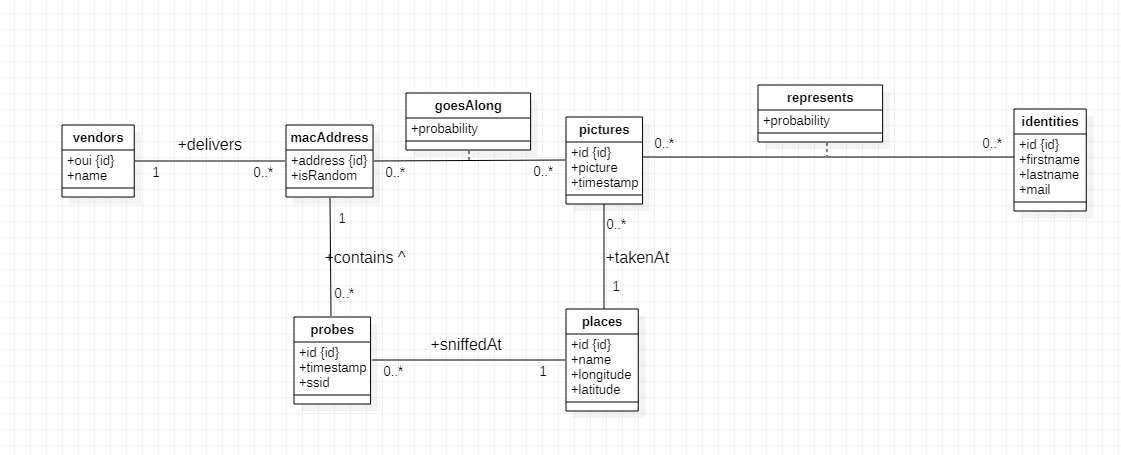
\includegraphics[width=12cm]{images/proto-3.png}
	\caption{Troisième version entité-association}
	\label{fig:arealytics}
\end{figure}

Le problème susmentionné a été résolu en détachant l’identité de l’adresse MAC. Seul la photo y est attachée, et
c’est maintenant le lien entre une adresse et une image qui est pondéré.

\section{API rest}

Pour des raisons d’évolutivité, de sécurité et de workflow, il a été décidé de développer une API pour interroger la
base de donnée depuis les clients. Ainsi, la responsabilité d’effectuer la grande partie de la logique métier pourra
être distribuée au serveur.

\section{L'API WiFace}

Afin de développer un projet plus évolutif, sécurisé, et scalable, il a été décidé d'implémenter une API rest permettant les opérations CRUD et d'autres
traitement sur les entités présentée dans la section ~\ref{sec:database}.

La liste des routes est donnée en annexe de ce document.

\section{Le client Raspberry}

\section{Algorithme PP2I}